\documentclass[draft]{article}

\usepackage{amsmath}
\usepackage{amsfonts}
\usepackage{graphicx}
\usepackage{url}
\usepackage{color}

\graphicspath{ {figures/} }

\title{Classifying brain states induced by comlex visual stimuli}

\author{Andrew Floren\\
1 University Station, C0803\\
The University of Texas at Austin\\
Austin TX, 78712-1084 USA\\
afloren@mail.utexas.edu\\
(214) 384-2895\\}

\date{}

\bibliographystyle{acm}

\begin{document}

\maketitle

\begin{abstract}
In traditional fMRI experiments, investigators seekt o identify relationships between the measured BOLD signal and a carefully designed stimulus in order to tease out the purpose of particular brain regions.
Recently, a new trend has developed where researchers are instead looking to predict what stimulus was presented given the measured BOLD signal \cite{fmri-ml1,fmri-ml2,fmri-ml3}.
While successful, most of these experiments involve presenting static images from a limited number classes such as faces and places.
Then, the researchers try to classify which image or class of images was presented during each frame by analyzing the measured BOLD signal using machine learning classifiers.
We wanted to test to what extent it is possible to classify a subject's brain state while presenting more realistic stimuli.
Further, we were interested to see what information could be gleaned from the BOLD signal beyond object categories.
\end{abstract}

\tableofcontents

\section{Introduction}
In traditional fMRI experiments, investigators seekt o identify relationships between the measured BOLD signal and a carefully designed stimulus in order to tease out the purpose of particular brain regions.
Recently, a new trend has developed where researchers are instead looking to predict what stimulus was presented given the measured BOLD signal \cite{fmri-ml1,fmri-ml2,fmri-ml3}.
While successful, most of these experiments involve presenting static images from a limited number classes such as faces and places.
Then, the researchers try to classify which image or class of images was presented during each frame by analyzing the measured BOLD signal using machine learning classifiers.
We wanted to test to what extent it is possible to classify a subject's brain state while presenting more realistic stimuli.
Further, we were interested to see what information could be gleaned from the BOLD signal beyond object categories.

\section{Methods}

\subsection{Stimulus}
We developed a virtual reality environment similar to many popular first person video games.
The stimuli is dunamically rendered and presented from the pointof view of a camera moving through this virutal environmentw hile characters are presented.
An exmaple frame from this sequence is presented in fgure 1.
The stimulus is a classic block design, in which the viewpoint moves for 15 seconds through a town, then pauses for 15 seconds amidst a group of characteres that fade into view.
The camera isconstantlymoving and the characters are animated such that the presented scene is never static.
The number of characters varies from one to six in each presentation in a quasi-random fashion.
Each run consists of 24 blocks of 15 seconds each., half with characters and half moving through an empty town.
4 to 6 runs were obtained in each scanning session.

\subsection{fMRI}
We collected whole brain scans using a GRAPPA-accelerated EPI, with a 2.5 second TR and 2.5 mm cubic voxels on 40 slices that covered the majority of each subjects brain (see figure \ref{fig:rx}).

\begin{figure}[!htbp]
\centering
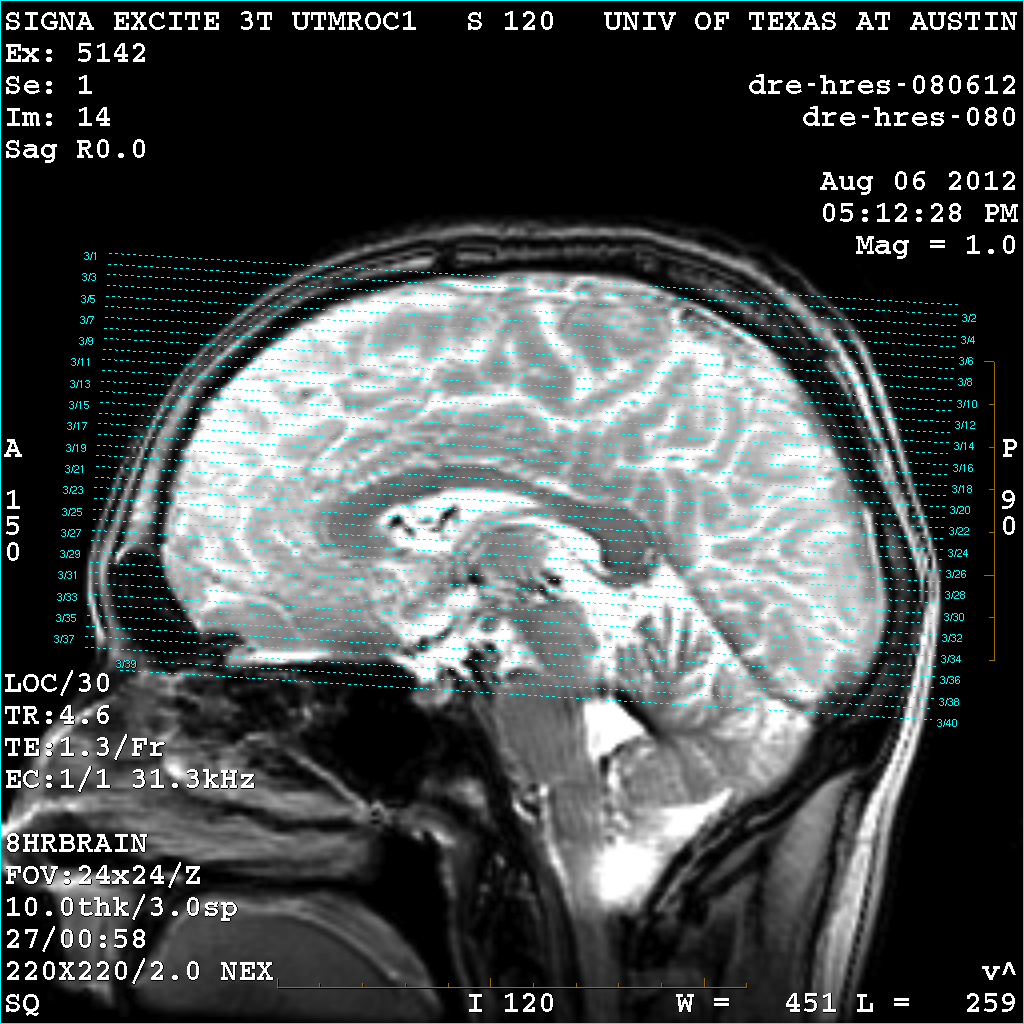
\includegraphics[width=0.5\textwidth]{rx}
\caption{An example perscription from one of the subjects.}
\label{fig:rx}
\end{figure}

\subsection{Preprocessing}
We performed motion compensation ad slice timing corrections. 
Additionally, we applied a Wiener filter using a generic difference-of-gamma HRF \cite{glover-ref} to shift the peak response in time so that it is aligned with the stimulus that caused it.
Finally, we reduce the dimensionality of the problem by masking out a subset of he volume using a harmonic power analysis.
We selected N (~3000) voxels with the greatest power at the frquency of the block alternation and its harmonics.
In other words, we selected the vosels that responded in any fashion that covaried with the stimulus alternations.
Thus, the selection was based only on the alternation between presentation of characters and the empty town, without regard to the number of characters.

\subsection{Classification}
Using the timer series of data from these voxels, we trained a linear SVM and a feed forward neural network.
Thes algorithms were trained and validated using a cross-fold approach \cite{crossfold}.
Each frame or point in the time series was treated as a separate data point instead of averaging across the block.
However, data points from the same block were not allowed to be split across the training and test set in order to avoid issues with noise correlations causing overly optimistic performace estimates.

\section{Results}

\section{Conclusions}

Earlier, we presnted this new trend in brain sate classification as a departure from tradiional fMRI experiments which seek to identify the purpose or function of particular brain regions.
However, it is important to note that through sensitivity analysis these machinelearning classifiers can be repurposed for just that goal.
If a region of the brain is highly important for accurately predicting the presence of a particular stimulus then it logically follows that that region must somehow be involved in the processing of that stimulus.
Furthermore, multi-voxel non-linear machine learning classifiers can potentially identify much more complex interactions between brain regions than the simple GLM.


\bibliography{bib}

\end{document}
